\documentclass{beamer}

\usepackage[T1]{fontenc}
\usepackage[utf8]{inputenc}
\usepackage[frenchb]{babel}
\usepackage{eurosym}

\usepackage{graphicx}


\newcommand\host{{\it host}\,}
\newcommand\device{{\it device}\,}


% --------- BEGIN STYLE BEAMER ---------
\usetheme{Madrid}
\definecolor{ECNBleu}{HTML}{102648}
\definecolor{ECNJaune}{HTML}{FAB600}

\setbeamercolor{frametitle}{bg=ECNBleu,fg=white} %le titre de la frame, en haut
\setbeamercolor{title in head/foot}{bg=ECNJaune,fg=ECNBleu} %barre bas, milieu
\setbeamercolor{author in head/foot}{bg=ECNBleu,fg=ECNJaune} %barre bas, gauche
\setbeamercolor{date in head/foot}{bg=ECNBleu,fg=ECNJaune} %barre bas, droit
\setbeamercolor{section in head/foot}{bg=ECNJaune,fg=ECNBleu} %haut gauche
\setbeamercolor{subsection in head/foot}{bg=ECNBleu,fg=ECNBleu} %haut droite
\setbeamercolor{title}{bg=ECNBleu,fg=white}
\setbeamercolor{block title}{fg=white,bg=ECNBleu}

%\setbeamercolor{normal text}{bg=IUTBleuFonce} %texte
\setbeamercolor{item}{bg=ECNBleu}
\setbeamercolor{subitem}{bg=ECNJaune}
\setbeamercolor{description item}{fg=couleurEmph}
\setbeamercolor{section in toc}{fg=ECNBleu}
%\setbeamercolor{subsubitem}{bg=IUTBleuFonce}

%structure (eq emph dans beamer)
\setbeamercolor{emph}{fg=couleurEmph}
% ----------------------------

\usepackage{listings}

\lstdefinestyle{customc}{
  belowcaptionskip=1\baselineskip,
  breaklines=true,
  frame=L,
  xleftmargin=\parindent,
  language=C,
  showstringspaces=false,
  basicstyle=\tiny\ttfamily,
  keywordstyle=\bfseries\color{green!40!black},
  commentstyle=\itshape\color{purple!40!black},
  identifierstyle=\color{blue},
  stringstyle=\color{orange},
}

\lstset{escapechar=@,style=customc}

\newenvironment<>{questionblock}[1]{%
\setbeamercolor{block title}{bg=ECNJaune,fg=ECNBleu}%
\begin{block}#2{#1}}{\end{block}}

\title[GPGPU]{Programmation sur Processeur Graphique}
\subtitle[\ldots]{
---\\Partie 2 : Allocation des données et exécution d'un kernel}
\author[P.-E. Hladik]{Pierre-Emmanuel Hladik\\\tiny pierre-emmanuel.hladik@ec-nantes.fr}
\institute[Centrale Nantes]{}
\date{\today}

\begin{document}

 \frame{\titlepage}

%%%%%%%%%%%%%%%%%%%%%%%%%%%
%%%%%%%%%%%%%%%%%%%%%%%%%%%
\section{Introduction à la programmation parallèle}
\section{Allocation des données et exécution d'un kernel}
%%%%%%%%%%%%%%%%%%%%%%%%%%%
\begin{frame}{Plan}
\tableofcontents[sections={1-4}, currentsection, hideothersubsections]
\end{frame}
%%%%%%%%%%%%%%%%%%%%%%%%%%%
\section{Kernel à plusieurs dimensions}

%%%%%%%%%%%%%%%%%%%%%%%%%%
\begin{frame}[plain]
\frametitle{Structure d'un programme C en CUDA}

\begin{block}{\host et \device}
\begin{itemize}
	\item  \host = CPU
	\item  \device = GPU
\end{itemize}
\end{block}

\begin{block}{Principe d'exécution : fonction et kernel}
\center	
\includegraphics[scale=0.5]{./figures-pdf/execution}
\end{block}
\end{frame}
%%%%%%%%%%%%%%%%%%%%%%%%%%
%\begin{frame}[plain]
%\frametitle{Mémoire unifiée}
%
%
%\begin{block}{CUDA Unified Memory (UM)}
%\begin{itemize}
%	\item  Espace d'adressage mémoire unique accessible à la fois depuis l'\host et le \device
%	\item  Le matériel/logiciel gère  la migration des données entre l'\host et le \device en maintenant
%la cohérence entre eux
%\end{itemize}
%\end{block}
%\center
%	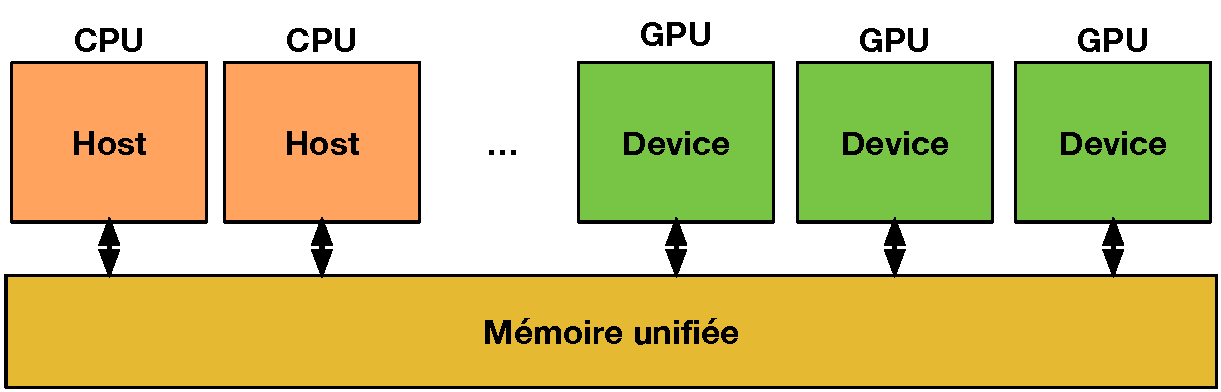
\includegraphics[scale=0.5]{./figures-pdf/uniform_memory}
%\end{frame}
%%%%%%%%%%%%%%%%%%%%%%%%%%
\begin{frame}[plain, fragile]
\frametitle{Exemple avec une addition vectorielle}
\center
	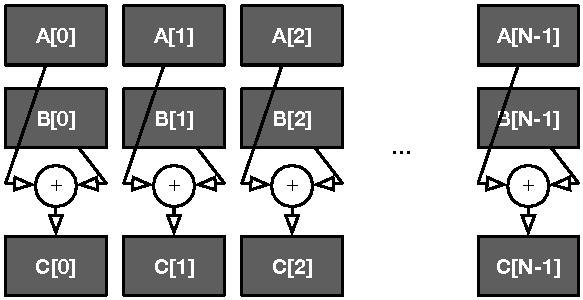
\includegraphics[scale=0.5]{./figures-pdf/add}
	  \begin{lstlisting}[language=C]
// Compute vector sum C = A + B
void vecAdd (float *h_A , float *h_B , float * h_C , int n)
{
  int i;
  for (i = 0; i<n; i++) {
    h_C [i] = h_A [i] + h_B [i];
  }
}

int main()
{
  // Memory allocation for for h_A , h_B , and h_C
  // I/O to read  h_A and h_B , N elements
  ...
  vecAdd (h_A , h_B , h_C , N);
}
	   \end{lstlisting}
	
\end{frame}
%%%%%%%%%%%%%%%%%%%%%%%%%%
\begin{frame}[plain, fragile]
\frametitle{Cas pratique : le collectif vu comme un GPU}

      \center
	
\includegraphics[scale=0.2]{./figures-pdf/groupe}
	
	id groupe + id thread => quel code écrire ?
	
\end{frame}

%%%%%%%%%%%%%%%%%%%%%%%%%%
\begin{frame}[plain, fragile]
\frametitle{Structure basique d'un code CUDA}
      \begin{block}{}
      \center
	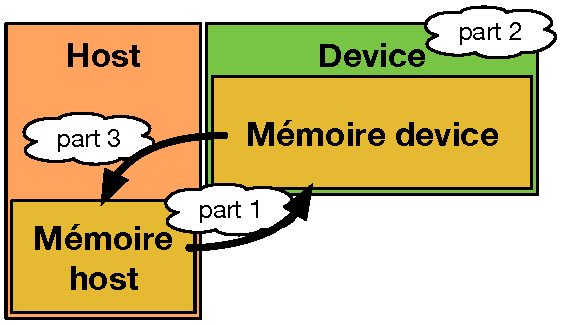
\includegraphics[scale=0.4]{./figures-pdf/principe}
	\end{block}  

  
	  \begin{lstlisting}[language=C]
#include <cuda.h>
void vecAdd(float *h_A, float *h_B, float *h_C, int n)
{
   int size = n* sizeof(float); 
   float *d_A, *d_B, *d_C;
   // Part 1
   // Allocate device memory for A, B, and C
   // copy A and B to device memory 

   // Part 2
   // Kernel launch code - the device performs the actual vector addition

   // Part 3
   // copy C from the device memory
   // Free device vectors
}
	   \end{lstlisting}

\end{frame}
%%%%%%%%%%%%%%%%%%%%%%%%%%
\begin{frame}[plain, fragile]
\frametitle{Allocation mémoire : cudaMalloc}

	  \begin{lstlisting}[language=C]
#include <cuda.h>
void vecAdd(float *h_A, float *h_B, float *h_C, int n)
{
   int size = n* sizeof(float); 
   float *d_A, *d_B, *d_C;
   // Allocate device memory for A, B, and C
   cudaMalloc((void **) &d_A, size);
   cudaMalloc((void **) &d_B, size);
   cudaMalloc((void **) &d_C, size);
   
   // copy A and B to device memory 

   // Part 2
   // Kernel launch code - the device performs the actual vector addition

   // Part 3 
   // copy C from the device memory
   // Free device vectors
}
	   \end{lstlisting}

\end{frame}
%%%%%%%%%%%%%%%%%%%%%%%%%%
\begin{frame}[plain, fragile]
\frametitle{Désallocation mémoire : cudaFree}

	  \begin{lstlisting}[language=C]
#include <cuda.h>
void vecAdd(float *h_A, float *h_B, float *h_C, int n)
{
   int size = n* sizeof(float); 
   float *d_A, *d_B, *d_C;
   // Allocate device memory for A, B, and C
   cudaMalloc((void **) &d_A, size);
   cudaMalloc((void **) &d_B, size);
   cudaMalloc((void **) &d_C, size);
   
   // copy A and B to device memory 

   // Part 2
   // Kernel launch code - the device performs the actual vector addition

   // Part 3
   // copy C from the device memory
   // Free device vectors
   cudaFree(d_A); cudaFree(d_B); cudaFree(d_C);
}
	   \end{lstlisting}

\end{frame}
%%%%%%%%%%%%%%%%%%%%%%%%%%
\begin{frame}[plain, fragile]
\frametitle{Copie mémoire : cudaMemcpy}

	  \begin{lstlisting}[language=C]
#include <cuda.h>
void vecAdd(float *h_A, float *h_B, float *h_C, int n)
{
   int size = n* sizeof(float); 
   float *d_A, *d_B, *d_C;
   // Allocate device memory for A, B, and C
   cudaMalloc((void **) &d_A, size);
   cudaMalloc((void **) &d_B, size);
   cudaMalloc((void **) &d_C, size);
   
   // copy A and B to device memory 
   cudaMemcpy(d_A, h_A, size, cudaMemcpyHostToDevice);
   cudaMemcpy(d_B, h_B, size, cudaMemcpyHostToDevice);

   // Part 2
   // Kernel launch code - the device performs the actual vector addition

   // Part 3
   // copy C from the device memory
   cudaMemcpy(h_C, d_C, size, cudaMemcpyDeviceToHost);
   // Free device vectors
   cudaFree(d_A); cudaFree(d_B); cudaFree(d_C);
}
	   \end{lstlisting}

\end{frame}
%%%%%%%%%%%%%%%%%%%%%%%%%%
\begin{frame}[plain]
\frametitle{Kernel, grid, block et thread}
      \begin{block}{}
      \center
	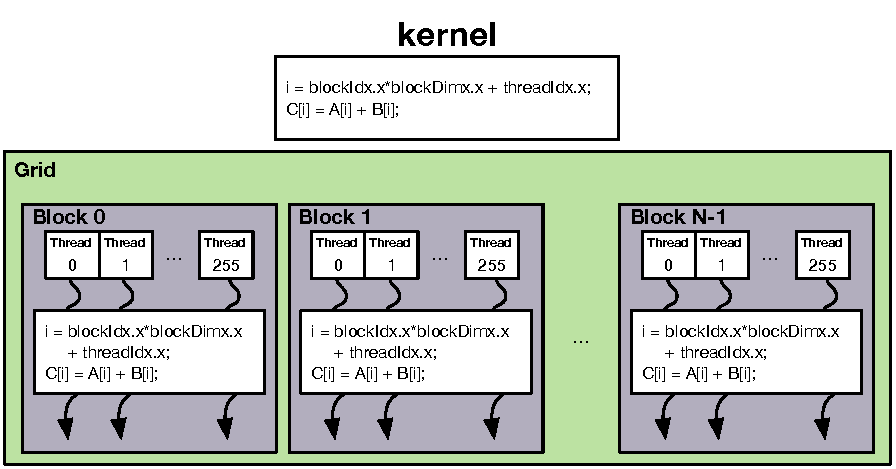
\includegraphics[scale=0.7]{./figures-pdf/kernel}
	
	\begin{itemize}
		\item Les threads d'un block coopèrent via une {\bf shared memory}, {\bf atomic operations} et {\bf barrier synchronization}
		\item les threads dans des blocs différents ne coopèrent pas
	\end{itemize}
	\end{block}  
\end{frame}
%%%%%%%%%%%%%%%%%%%%%%%%%%%
%\begin{frame}[plain]
%\frametitle{Execution}
%      \begin{block}{}
%	\begin{itemize}
%		\item Un thread peut être vu comme un processeur de type Von-Neumann
%		\item Tous les threads d'un bloc exécutent la même instruction (Single Program Multiple Data)
%	\end{itemize}
%      \center
%	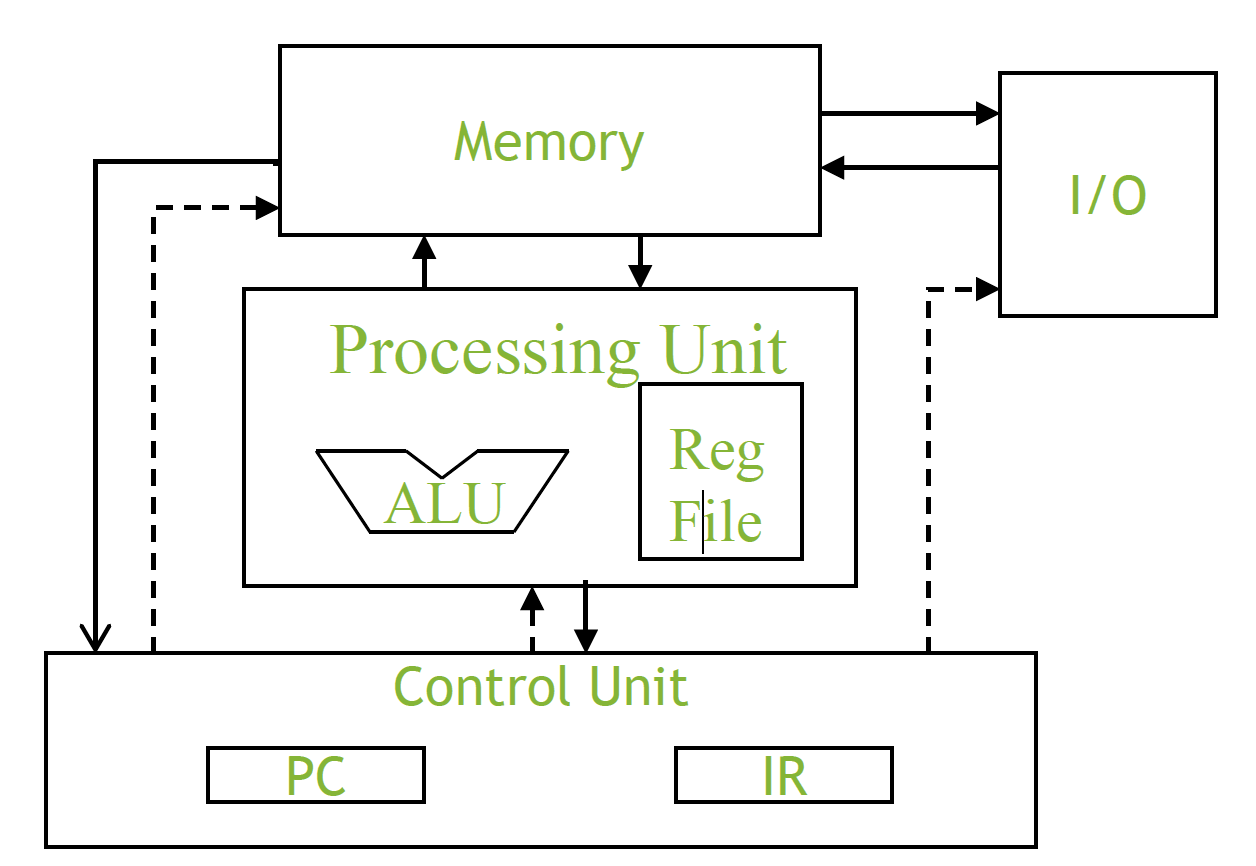
\includegraphics[scale=0.2]{./figures-pdf/von-neumann}
%	\end{block}  
%\end{frame}
%%%%%%%%%%%%%%%%%%%%%%%%%%
\begin{frame}[plain]
\frametitle{Thread index}
      \begin{block}{}
	\begin{itemize}
		\item Chaque thread a un index qui peut être utilisé pour manipuler les adresses mémoires et faire des choix d'exécution
	\end{itemize}
      \center
	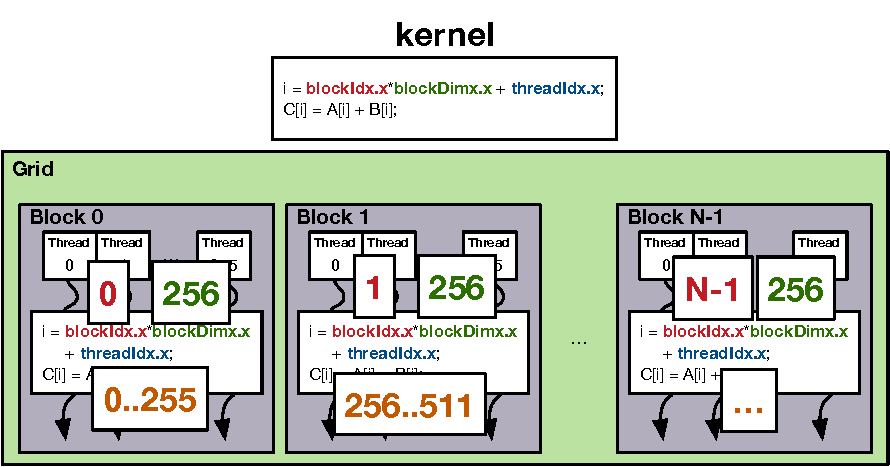
\includegraphics[scale=0.7]{./figures-pdf/index}
	\end{block}  
\end{frame}



%%%%%%%%%%%%%%%%%%%%%%%%%%
\begin{frame}[plain,fragile]
\frametitle{Définition d'un kernel en CUDA}

	  \begin{lstlisting}[language=C]
// Compute vector sum C = A + B
// Each thread performs one pair-wise addition

__global__
void vecAddKernel(float* A, float* B, float* C, int vectorSize)
{
  int kernelIdx = threadIdx.x + blockDim.x*blockIdx.x;
  if(i < vectorSize)
  {
    C[kernelIdx] = A[kernelIdx] + B[kernelIdx];
  }
}
	   \end{lstlisting}
\end{frame}
%%%%%%%%%%%%%%%%%%%%%%%%%%
\begin{frame}[plain,fragile]
\frametitle{Execution d'un kernel}

%	  \begin{lstlisting}[language=C]
%// Compute vector sum C = A + B
%// Each thread performs one pair-wise addition
%
%__global__
%void vecAddKernel(float* A, float* B, float* C, int n)
%{
%  int i = threadIdx.x + blockDim.x*blockIdx.x;
%  if(i<n) C[i] = A[i] + B[i];
%}
%
%void vecAdd(float* h_A, float* h_B, float* h_C, int n)
%{
%  // d_A, d_B, d_C allocations and copies omitted
%  // Run ceil((float)n/256.0) blocks of 256 threads each
%  int DimGrid = ceil((float)n/256.0);
%  int DimBlock = 256;
%  vecAddKernel<<<DimGrid,DimBlock>>>(d_A, d_B, d_C, n);
%}
%	   \end{lstlisting}


	  \begin{lstlisting}[language=C]
// Compute vector sum C = A + B
// Each thread performs one pair-wise addition

__global__
void vecAddKernel(float* A, float* B, float* C, int vectorSize)
{
  int kernelIdx = threadIdx.x + blockDim.x*blockIdx.x;
  if(kernelIdx < vectorSize)
  {
    C[kernelIdx] = A[kernelIdx] + B[kernelIdx];
  }
}

void vecAdd(float* h_A, float* h_B, float* h_C, int size)
{
  // d_A, d_B, d_C allocations and copies omitted
  // Run ceil((float)n/256.0) blocks of 256 threads each
  int number_of_blocks = ceil((float) size / 256.0);
  int number_of_threads_per_block = 256;
  vecAddKernel<<< number_of_blocks, number_of_threads_per_block >>>(d_A, d_B, d_C, n);
}
	   \end{lstlisting}
\end{frame}
%%%%%%%%%%%%%%%%%%%%%%%%%%
\begin{frame}[plain]
\frametitle{Thread index}
      \begin{block}{}
      \center
	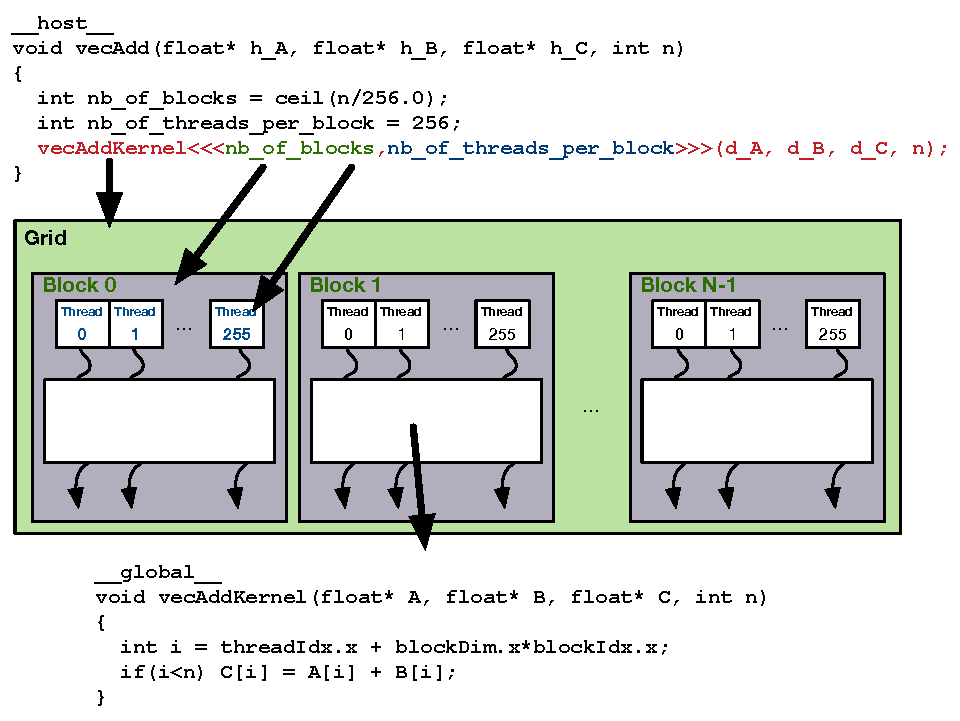
\includegraphics[scale=0.6]{./figures-pdf/nutshell}
	\end{block}  
\end{frame}

%%%%%%%%%%%%%%%%%%%%%%%%%%
\begin{frame}[plain]
\frametitle{Mots-clef en CUDA-C pour déclarer les fonctions}
\begin{table}[htdp]

\begin{center}
\begin{tabular}{|ll|c|c|}
\hline
 &&  exécuté sur & appelé par\\
\hline
{\tt \_\_device\_\_}& {\tt float DeviceFunc()} & device & device\\
{\tt \_\_global\_\_} & {\tt void  KernelFunc()} & device & host\\
{\tt \_\_host\_\_ }  & {\tt float HostFunc()} & host & host\\
\hline
\end{tabular}
\end{center}
\end{table}%
\begin{itemize}
	\item {\tt \_\_global\_\_} définit une fonction kernel
	\item Une fonction kernel doit retourner un {\tt void} (mais peut prendre ce que l'on veut en argument)
	\item {\tt \_\_device\_\_} et {\tt \_\_host\_\_} peuvent être utilisés conjointement pour avoir deux versions objet de la même fonction.
	\item {\tt \_\_host\_\_} est optionnel s'il est utilisé seul
\end{itemize}

\end{frame}
%%%%%%%%%%%%%%%%%%%%%%%%%%%
%\begin{frame}[plain]
%\frametitle{blockIdx et threadIdx}
%      \begin{block}{}
%	\begin{itemize}
%		\item Les index de block et de thread sont des variables à trois dimensions
%		\item Cela simplifie les adresses mémoires quand on travaille avec des données multidimentionelles (image, volumes, etc.)
%	\end{itemize}
%      \center
%	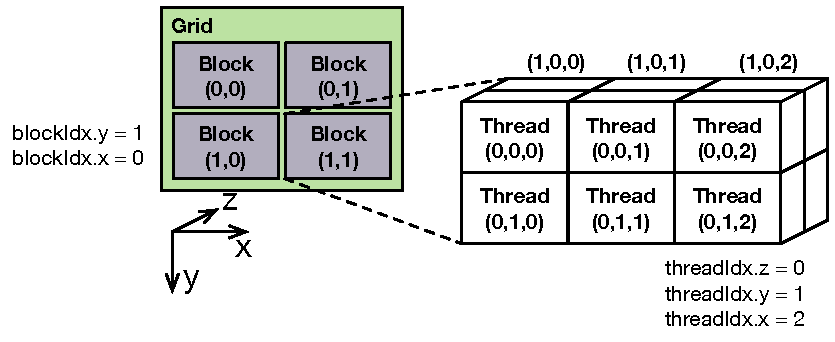
\includegraphics[scale=0.7]{./figures-pdf/indexDim}
%	\end{block}  
%\end{frame}
%%%%%%%%%%%%%%%%%%%%%%%%%%%
%\begin{frame}[plain,fragile]
%\frametitle{Execution d'un kernel 1D (multidim)}
%
%	  \begin{lstlisting}[language=C]
%void vecAdd(float* h_A, float* h_B, float* h_C, int n)
%{
%  // d_A, d_B, d_C allocations and copies omitted
%  // Run ceil((float)n/256.0) blocks of 256 threads each
%  dim3 DimGrid((n-1)/256 + 1, 1, 1);
%  dim3 DimBlock(256, 1, 1);
%  vecAddKernel<<<DimGrid,DimBlock>>>(d_A, d_B, d_C, n);
%}
%	   \end{lstlisting}
%\end{frame}
%%%%%%%%%%%%%%%%%%%%%%%%%%%

%%%%%%%%%%%%%%%%%%%%%%%%%%
\begin{frame}[plain, fragile]
\frametitle{Si on veut bien faire les choses : gestion des erreurs}

Toutes les fonctions de l'API CUDA retournent un code d'erreur (de type {\tt cudaError\_t}), il peut être utile de tester la valeur pour s'éviter de problème, par exemple :

 \begin{lstlisting}[language=C]
cudaError_t  err = cudaMalloc((void **) &d_A, size);

if (err != cudaSuccess)  {
   printf("%s in %s at line %d\n",   cudaGetErrorString(err), __FILE__,
   __LINE__);
   exit(EXIT_FAILURE);
}
	   \end{lstlisting}

\begin{alertblock}{}
Attention l'appel au kernel {\tt {<}{<}{<}...{>}{>}{>}()} n'est pas un appel de fonction et se fait de manière asynchrone. Il faut utiliser {\tt cudaGetLastError()} et surtout {\tt cudaDeviceSynchronize()} pour se synchroniser (voir TD pour plus de détails).
\medskip

{\bf Description :} {\tt Blocks until the device has completed all preceding requested tasks. cudaDeviceSynchronize() returns an error if one of the preceding tasks has failed.}
\end{alertblock}
\end{frame}

%%%%%%%%%%%%%%%%%%%%%%%%%%
\begin{frame}[plain]
\frametitle{Un peu de pratique avec le TD2}

\begin{block}{Objectifs}
\begin{itemize}
	\item Allocation mémoire et écriture d'un premier kernel
	\item Gérer les erreurs
	\item Se casser les dents sur la gestion de la mémoire structurée
\end{itemize}
\end{block}
\end{frame}
%%%%%%%%%%%%%%%%%%%%%%%%%%


\end{document}